Consider following unity gain feedback system. 
\begin{center}
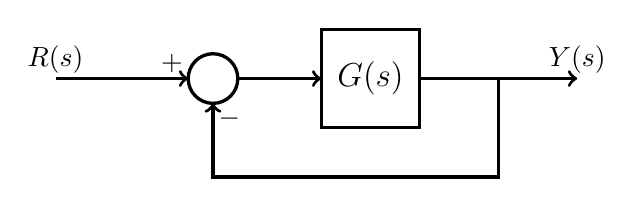
\begin{tikzpicture}[scale=1,inner sep=0pt,outer sep=0pt,very thick,
sysblock/.style={draw,rectangle,inner sep=2pt,minimum width=1.25cm,minimum height=1.25cm,inner sep=4pt, very thick}]
\draw (2,0) node[draw,circle] (sum1) {$\rule{0pt}{18pt}$};
\draw (4,0) node[sysblock] (G) {\large $G(s)$};
\draw[->] (0,0) node[above=2pt] {$R(s)$} -- (sum1.180) node[above left=2pt] {$+$};
\draw[->] (sum1.0)  -- (G.180);
\draw[->] (G.0) -- ++(2,0) node[above=2pt] {$Y(s)$};
\draw[->] (G.0) ++(1,0) -- ++(0,-1.25) -| (sum1.-90) node[below right=2pt] {$-$};
\end{tikzpicture}
\end{center}
The following is the Bode plot of $G(s)$, which is stable.\vspace{-.1in}
\begin{center}
\includegraphics[width=4in]{\mainfolder/LectureNotes/\lecturefolder/HomeworkProblems/Problem05/bode2.pdf}
\end{center}

\begin{enumerate}[(a)]
\item What is the gain margin $\GMdB$?
\item What is the phase margin $\PM$?
\item Which of the following is the correct Nyquist plot?\\
\begin{minipage}{2.5in}
\begin{enumerate}
\item[(i)]  \parbox[c]{2in}{\includegraphics[width=2in]{\mainfolder/LectureNotes/\lecturefolder/HomeworkProblems/Problem05/nyquist2.pdf}}
\item[(ii)]  \parbox[c]{2in}{\includegraphics[width=2in]{\mainfolder/LectureNotes/\lecturefolder/HomeworkProblems/Problem05/nyquist3.pdf}}
\end{enumerate}
\end{minipage}
\begin{minipage}{2.5in}
\begin{enumerate}
\item[(iii)]  \parbox[c]{2in}{\includegraphics[width=2in]{\mainfolder/LectureNotes/\lecturefolder/HomeworkProblems/Problem05/nyquist1.pdf}}
\item[(iv)]  \parbox[c]{2in}{\includegraphics[width=2in]{\mainfolder/LectureNotes/\lecturefolder/HomeworkProblems/Problem05/nyquist4.pdf}}
\end{enumerate}
\end{minipage}
\item Is the closed-loop system stable?
\item If the closed loop system is stable, what is the maximum delay that can be tolerated (i.e. a change of the open loop system to $e^{-sT_{d}}G(s)$) before the closed loop system becomes unstable?
\end{enumerate}
